\documentclass[14pt,xcolor=pdftex,dvipsnames,table]{beamer}\usepackage[]{graphicx}\usepackage[]{color}
%% maxwidth is the original width if it is less than linewidth
%% otherwise use linewidth (to make sure the graphics do not exceed the margin)
\makeatletter
\def\maxwidth{ %
  \ifdim\Gin@nat@width>\linewidth
    \linewidth
  \else
    \Gin@nat@width
  \fi
}
\makeatother

\definecolor{fgcolor}{rgb}{0.345, 0.345, 0.345}
\newcommand{\hlnum}[1]{\textcolor[rgb]{0.686,0.059,0.569}{#1}}%
\newcommand{\hlstr}[1]{\textcolor[rgb]{0.192,0.494,0.8}{#1}}%
\newcommand{\hlcom}[1]{\textcolor[rgb]{0.678,0.584,0.686}{\textit{#1}}}%
\newcommand{\hlopt}[1]{\textcolor[rgb]{0,0,0}{#1}}%
\newcommand{\hlstd}[1]{\textcolor[rgb]{0.345,0.345,0.345}{#1}}%
\newcommand{\hlkwa}[1]{\textcolor[rgb]{0.161,0.373,0.58}{\textbf{#1}}}%
\newcommand{\hlkwb}[1]{\textcolor[rgb]{0.69,0.353,0.396}{#1}}%
\newcommand{\hlkwc}[1]{\textcolor[rgb]{0.333,0.667,0.333}{#1}}%
\newcommand{\hlkwd}[1]{\textcolor[rgb]{0.737,0.353,0.396}{\textbf{#1}}}%

\usepackage{framed}
\makeatletter
\newenvironment{kframe}{%
 \def\at@end@of@kframe{}%
 \ifinner\ifhmode%
  \def\at@end@of@kframe{\end{minipage}}%
  \begin{minipage}{\columnwidth}%
 \fi\fi%
 \def\FrameCommand##1{\hskip\@totalleftmargin \hskip-\fboxsep
 \colorbox{shadecolor}{##1}\hskip-\fboxsep
     % There is no \\@totalrightmargin, so:
     \hskip-\linewidth \hskip-\@totalleftmargin \hskip\columnwidth}%
 \MakeFramed {\advance\hsize-\width
   \@totalleftmargin\z@ \linewidth\hsize
   \@setminipage}}%
 {\par\unskip\endMakeFramed%
 \at@end@of@kframe}
\makeatother

\definecolor{shadecolor}{rgb}{.97, .97, .97}
\definecolor{messagecolor}{rgb}{0, 0, 0}
\definecolor{warningcolor}{rgb}{1, 0, 1}
\definecolor{errorcolor}{rgb}{1, 0, 0}
\newenvironment{knitrout}{}{} % an empty environment to be redefined in TeX

\usepackage{alltt}

% Specify theme
\usetheme{Madrid}
% See deic.uab.es/~iblanes/beamer_gallery/index_by_theme.html for other themes
\usepackage{caption}
\usepackage[comma, sort&compress]{natbib}
\usepackage{graphicx}
\usepackage{amsmath}
\bibliographystyle{agsm}
% Specify base color
\usecolortheme[named=OliveGreen]{structure}
% See http://goo.gl/p0Phn for other colors

% Specify other colors and options as required
\setbeamercolor{alerted text}{fg=Maroon}
\setbeamertemplate{items}[square]

% Title and author information
\title{Introduction to Regression and OLS}
\author{Rob Hayward}
\IfFileExists{upquote.sty}{\usepackage{upquote}}{}
\begin{document}

\begin{frame}
\titlepage
\end{frame}

\begin{frame}{Outline}
\tableofcontents
\end{frame}



\begin{frame}{Modelling}
The model
\begin{block}{}
$y_t = \alpha + \beta x_t + \varepsilon_t$
\end{block}
\pause
Where 
\begin{itemize}[<+-| alert@+>]
\item $y_t$ is the dependent variable
\item $\alpha$ is an intercept or constant
\item $x_t$ is the explanatory or independent variable(s)
\item $\beta$ is the key relationship
\item $\varepsilon_t$ is the error that covers omitted variables, measurement error and other stochastic or random elements
\end{itemize}
\end{frame}

\begin{frame}{Modelling}
The model
\begin{block}{}
$y_t = \alpha + \beta x_t + \varepsilon_t$
\end{block}

\pause

Where 
\begin{itemize}[<+-| alert@+>]
\item $y_t$ is the inflation rate
\item $\alpha$ is an intercept or constant
\item $x_t$ is the unemployment rate
\item $\beta$ is the relationship between the inflation rate and the unemployment rate
\item $\varepsilon_t$ is all the other factors that affect the inflation rate
\end{itemize}
\end{frame}


\begin{frame}{Caution!}
\begin{block}{}
\begin{quote} ``Essentially all models are wrong, but some are useful''
\end{quote} %citep[p. 424]{Box}
\end{block}
\end{frame}



\begin{frame}{Scattergram}
\begin{knitrout}
\definecolor{shadecolor}{rgb}{0.969, 0.969, 0.969}\color{fgcolor}
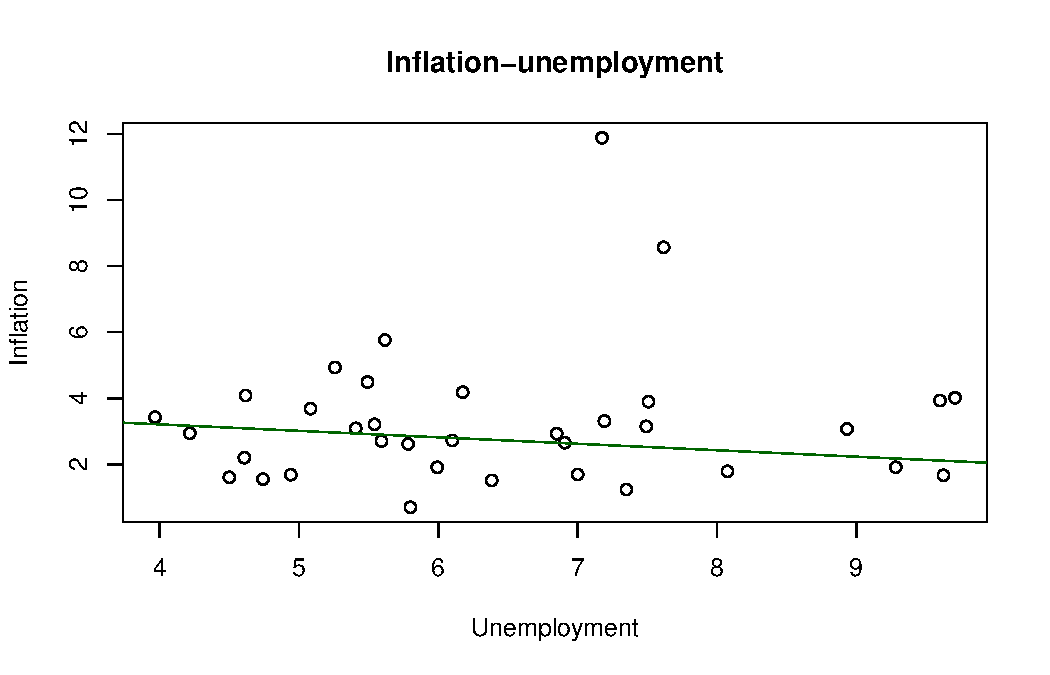
\includegraphics[width=\maxwidth]{figure/scatter-1} 

\end{knitrout}
\end{frame}


\begin{frame}{R Squared (p. 13)}
The total variance of the dependent variable is called the total sum of squares (TSS).  This can be split into 
\begin{itemize}[<+-| alert@+>]
\item Explained sum of squares or sum of squares of the regression (ESS)
\item Residual sum of squares (RSS)
\end{itemize}
\pause
\begin{align*}
R^2 &= 1 - \frac{RSS}{TSS} = 1 - \frac{RSS}{RSS + ESS}\\
R^2 &= 1 - \frac{\hat{\varepsilon}'\hat{\varepsilon}}{(y - \bar{y})'(y - \bar{y})}
\end{align*}
\begin{equation}
u = \hat{\varepsilon}
\end{equation}
\end{frame}

\begin{frame}{Adjusted R Squared (p. 13)}
The $R^2$ can be considered a measure of \emph{goodness of fit}.  However, the more variables that you add the smaller the $R^2$. The \emph{Adjusted R Squared} ($\bar{R}^2$) will make a penalty for adding variables. 

\begin{equation}
\bar{R}^2 = 1 - (1 - R^2) \times \frac{(T - 1)}{(T - K)}
\end{equation}
where $T$ is the total number of observations and $K$ is the number of variables. 
\end{frame}


\section{Confidence intervals on coefficients}
\begin{frame}{Coefficient Estimates}
Remember that the estimates of the coefficients will depend on the sample
\begin{itemize}[<+-| alert@+>]
\item A different sample will give a different estimate
\item We want to know how reliable the estimates will be under different samples
\item $\beta$ is a random variable.  If OLS (\emph{Gauss-Markov} assumptions hold)
\begin{itemize}
\item $\hat{\beta_1} \sim N (\beta_1, \sigma_{\beta_1}^2)$
\end{itemize}
\pause
If we assume a normal distribution we can carry out hypothese tests about coefficients like $\beta_1$
\end{itemize}
\end{frame}


\end{document}
